\documentclass[border=3mm]{standalone}

\usepackage{tikz}
\usetikzlibrary{arrows.meta}

\begin{document}
	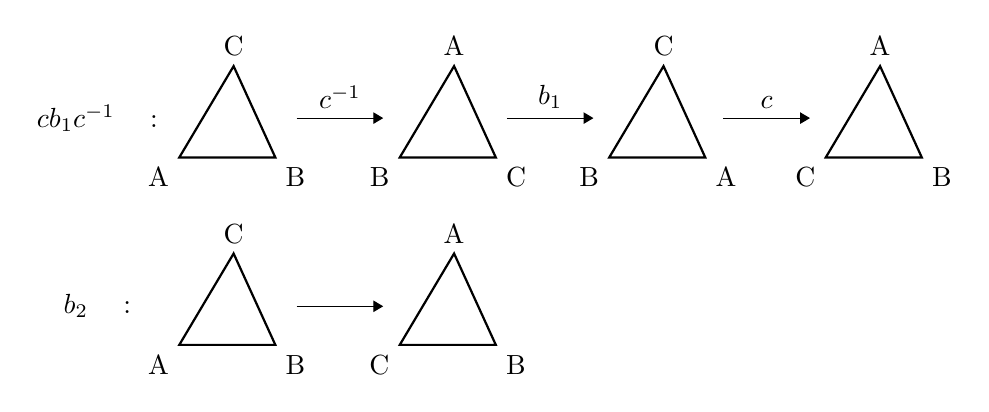
\begin{tikzpicture}
		\draw[thick] (-3.1,1.7) node[above] {C} -- (-2.57,0.54) node[below right] {B} -- (-3.79,0.54) node[below left] {A} -- cycle;
		\draw[thick] (-0.3,1.7) node[above] {A} -- (0.23,0.54) node[below right] {C} -- (-0.99,0.54) node[below left] {B} -- cycle;
		\draw[thick] (2.36,1.7) node[above] {C} -- (2.89,0.54) node[below right] {A} -- (1.67,0.54) node[below left] {B} -- cycle;
		\draw[thick] (5.11,1.7) node[above] {A} -- (5.64,0.54) node[below right] {B} -- (4.42,0.54) node[below left] {C} -- cycle;
		\draw[thick] (-3.1,-0.68) node[above] {C} -- (-2.57,-1.84) node[below right] {B} -- (-3.79,-1.84) node[below left] {A} -- cycle;
		\draw[thick] (-0.3,-0.68) node[above] {A} -- (0.23,-1.84) node[below right] {B} -- (-0.99,-1.84) node[below left] {C} -- cycle;
		\draw[-Triangle] (-2.3,1.04) -- (-1.2,1.04) node[above,midway] {$c^{-1}$};
		\draw[-Triangle] (0.37,1.04) -- (1.47,1.04) node[above,midway] {$b_{1}$};
		\draw[-Triangle] (3.12,1.04) -- (4.22,1.04) node[above,midway] {$c$};
		\draw[-Triangle] (-2.3,-1.35) -- (-1.2,-1.35) node[above,midway] {};
		\node at (-4.83,1.04) {$cb_1c^{-1} \quad :$};
		\node at (-4.83,-1.35) {$b_2 \quad :$};
	\end{tikzpicture}
\end{document}